\chapter{Att skriva loggbok}

\section{Loggbok}

\subsection{Ändamål}
\harec{c}{3.3.2}{3.3.2}
\index{stationsdagbok}
\index{loggbok}

Dina radioförbindelser och övriga händelser med radiostationen bör
antecknas i en \emph{stationsdagbok} även känd som \emph{loggbok}.
Tidigare fanns myndighetskrav på att föra loggbok, men det finns inte numer.

Amatörradioverksamheten bygger på förtroende och då är det viktigt att själv
kunna dokumentera sin verksamhet till exempel i störningssituationer med mera.
Loggen används också för att kunna visa när man har varit aktiv.

Helt i eget intresse är det ju också trevligt med en loggbok.
Tänk bara på hur bra det är att ha alla underlag för tävlingar och diplom
med mera dokumenterade.

\subsection{Kunna visa hur man för en loggbok}
\harec{c}{3.3.1}{3.3.1}

I bild \ref{loggblad} visas ett exempel på hur en förenklad loggsida kan se ut
med ett par radioförbindelser (QSO) inskrivna.

Fundera på följande:
\begin{enumerate}
\item Halv tre på eftermiddagen den tionde oktober gör Arne (SM6XYZ)
  ett allmänt anrop på den lokala repeatern på 2-metersbandet.
  Eva (SM6ZYX) som är på väg hem från skolan svarar.
  Arne berättar att han precis har byggt sitt nya slutsteg på 25~W
  färdigt och frågar Eva om det hörs någon skillnad när han kopplar ur det.
  Efter lite småprat om allt möjligt säger de 73 till varandra och då har det
  gått sju minuter sen de började.
  Fyll i loggboken åt Arne!
\item Gör ett låtsas-QSO med en kurskamrat.
  Bokstavera era ''anropssignaler''.
  För in i loggen.
\end{enumerate}

% \newpage
\begin{table}[h!]
  \vspace*{2cm}
  
  \qquad
  \begin{tabular}{|c|c|c|c|c|c|c|c|c|c|c|}
    \hline
    & band / & \multicolumn{2}{|c|}{tid-UTC} & anrops- & \multicolumn{2}{|c|}{RST} & &
                                                                                       \multicolumn{2}{|c|}{QSL} & \\
    datum & frekvens & start & slut & signal & sänt & fick & namn och QTH & s & m & anmärkning \\
    \hline
    \hline
    20171021 & 80 & 06:55 & 07:13 & SK0HQ & 59 & 59 & Anders & & & HQ-nätet \\
    \hline
    20171021 & 80 & 07:15 & 07:38 & SM0ZXY & 579 & 559 & Eva Sollentuna & & & \\
    \hline
    & & & & & & & & & & \\
    \hline
    & & & & & & & & & & \\
    \hline
  \end{tabular}
  \caption{Exempel på loggblad}
  \label{tab:loggblad}
\end{table}

\subsection{Föra in data}
\harec{c}{3.3.3}{3.3.3}

Det man skriver upp i loggen är:
\begin{itemize}
  \item Tiden i början och i slutet av förbindelsen. Glöm inte datum!
  \item motstationens anropssignal
  \item din effekt (ineffekt, PEP eller utstrålad effekt)
  \item frekvensband, ev frekvens
  \item sändningsslag (FM, SSB, CW, paketradio etc)
  \item uppgift om varifrån man sände (eget QTH)
  \item signalrapporter (rapportkoder).
\end{itemize}

Allmänna uppgifter om motstationen, till exempel signalrapport, namn, QTH,
motpartens utrustning, QSL-adress och så vidare brukar också vara bra att ha med.

Man bör också skriva upp när man har gjort allmänt anrop, sänt ut
bärvåg för prov, experiment och annat som kan vara av intresse.

Om någon annan radioamatör använder din station ska du också skriva
upp hans/hennes namn och anropssignal.

\subsection{Rapportkoder}

Man blir ofta ombedd av motstationen att lämna en så kallad signalrapport på
dennes sändning.
Omvänt är det bra att få en signalrapport på den egna sändningen.

För rapportering mellan radioamatörer används RST-koden.

För lyssnarrapporter till exempel till rundradiostationer, förekommer ett
kodsystem, som kallas för SINPO eller SINPFEMO. Se bilaga \ref{Rapportkoder}.

%% \begin{figure*}[b]
%%   \begin{center}
%%     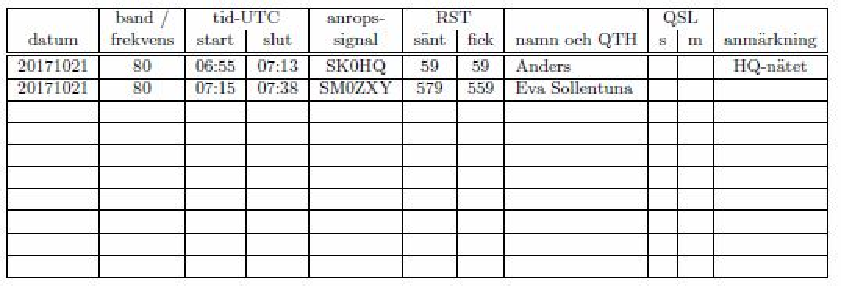
\includegraphics[width=0.8\textwidth]{images/cropped_pdfs/bild_15_1-01.pdf}
%%     \caption{Exempel på loggblad}
%%     \label{loggblad}
%%   \end{center}
%% \end{figure*}
% \mediumfig[0.7]{images/cropped_pdfs/bild_15_1-01.pdf}{Exempel på loggblad}{loggblad}


%%% Local Variables: ***
%%% mode: latex ***
%%% TeX-master: "../koncept-tryck.tex"  ***
%%% ispell-local-dictionary: "swedish"  ***
%%% End: ***